\documentclass[12 pt]{article}        	%sets the font to 12 pt and says this is an article (as opposed to book or other documents)
\usepackage{amsfonts, amssymb}					% packages to get the fonts, symbols used in most math
\usepackage{graphicx}
  
%\usepackage{setspace}               		% Together with \doublespacing below allows for doublespacing of the document

\oddsidemargin=-0.5cm                 	% These three commands create the margins required for class
\setlength{\textwidth}{6.5in}         	%
\addtolength{\voffset}{-20pt}        		%
\addtolength{\headsep}{25pt}           	%



\pagestyle{myheadings}                           	% tells LaTeX to allow you to enter information in the heading
\markright{Andrew Mayo\hfill \today \hfill}  
																									% and put the proposition number from the book
                                                	% LaTeX will put your name on the left, the date the paper 
                                                	% is generated in the middle 
                                                 	% and a page number on the right



\newcommand{\eqn}[0]{\begin{array}{rcl}}%begin an aligned equation - allows for aligning = or inequalities.  Always use with $$ $$
\newcommand{\eqnend}[0]{\end{array} }  	%end the aligned equation

%\doublespacing                         	% Together with the package setspace above allows for doublespacing of the document

\newcommand{\qed}[0]{$\square$}        	% make an unfilled square the default for ending a proof

\begin{document}												% end of preamble and beginning of text that will be printed 
\textbf{1 (a)} 
\[
  \frac{\partial{E(w)}}{\partial w_j} = 
  \sum_{i=1}^{N} (x_j)^{(i)} y^{(i)} (1 - \sigma(w^T x^{(i)}))
  - (x_j)^{(i)} \sigma(w^T x^{(i)}) 
  + (x_j)^{(i)} y^{(i)} \sigma(w^T x^{(i)})
\]
\[
  = \sum_{i=1}^{N} (x_j)^{(i)} y^{(i)} 
  - (x_j)^{(i)} \sigma(w^T x^{(i)}) 
\]
\[
  \frac{\partial^2 E(w)}{\partial (w_j)^2}
  = - \sum_{i=1}^{N} (x_j)^{(i)} \sigma(w^T x^{(i)}) (1 - \sigma(w^T x^{(i)})) (x_j)^{(i)}
\]
\[
  \frac{\partial^2 E(w)}{\partial w_j w_k}
  = - \sum_{i=1}^{N} (x_j)^{(i)} \sigma(w^T x^{(i)}) (1 - \sigma(w^T x^{(i)})) (x_k)^{(i)}
\]
Let $ X \in \mathbb{R}^{n \times m} $ be the design matrix 
and $ w \in \mathbb{R}^m $ be the weight vector, 
where $ n $ is the number of observations
and $ m $ is the number of features. 
Let $ \odot $ express the Hadamard product of its operands. 
We can express the second-order partial derivatives in matrix form as 
\[
  X^T diag[ - \sigma(Xw) \odot (1 - \sigma(Xw)) ] X
\]
which gives us our Hessian matrix. \\ \\

\textbf{1 (b)} Let $ x, z \in \mathbb{R}^m $. Then
\[
  (x^T z)(x^T z) = 
  \sum_{i = 1}^{N} z_i x_i \sum_{j=1}^{N}x_j z_j
  = \sum_{i = 1}^{N} \sum_{j=1}^{N} z_i x_i x_j z_j
  = (x^T z)^2
\]
Consider
\[
  z^T X^T diag[ \sigma(Xw) \odot (1 - \sigma(Xw)) ] X z
\]
Let $ D $ represent $ X^T diag[ \sigma(Xw) (1 - \sigma(Xw)) ] X $. $ D \in \mathbb{R}^{ m \times m }$. 
Let $ D_i $ be a column of $ D $ and $ D^{(j)} $ be a row of $ D $.
we can now express the above as 
\[
  - \sum_{i=1}^{m} [ \sum_{j=1}^{m} z_j (D_i)^{(j)} ] z_i
\]
\[
  = - \sum_{i=1}^{m} [ \sum_{j=1}^{m} z_j ((D_i)^{(j)})^{\frac{1}{2}} ((D_i)^{(j)})^{\frac{1}{2}} ] z_i
  = - \sum_{i=1}^{m} \sum_{j=1}^{m} z_j ((D_i)^{(j)})^{\frac{1}{2}} ((D_i)^{(j)})^{\frac{1}{2}} z_i
\]
Since in general $ \sum_{i = 1}^{N} \sum_{j=1}^{N} z_i x_i x_j z_j  = (x^T z)^2 \ge 0 $, 
\[
  \sum_{i=1}^{m} \sum_{j=1}^{m} z_j ((D_i)^{(j)})^{\frac{1}{2}} ((D_i)^{(j)})^{\frac{1}{2}} z_i \ge 0
\]
therefore 
\[
  - \sum_{i=1}^{m} [ \sum_{j=1}^{m} z_j (D_i)^{(j)} ] z_i \le 0 \; \square
\]
The Hessian matrix is negative semi-definite, and our original log-likelihood function is concave. \\ \\

\textbf{1 (c)} We can invert the sign of the log-lihelihood function to get a loss function. This gives us the Hessian matrix 
$ X^T diag[ \sigma(Xw) \odot (1 - \sigma(Xw)) ] X $. For the gradient of the loss function with respect to $ w $, 
we can take the partial derivative expression from \textbf{1 (a)}
\[
  \sum_{i=1}^{N} (x_j)^{(i)} y^{(i)} 
  - (x_j)^{(i)} \sigma(w^T x^{(i)})
\]
invert the sign, and express it in matrix form:
\[
  \nabla_w E = X^T \sigma(Xw) - X^T y
\]

So we the update for Newton's method is
\[
  w_{new} = w_{old} - H^{-1} \nabla_w E 
\]
\[
  w_{new} = w_{old} - \{X^T diag[ \sigma(Xw) \odot (1 - \sigma(Xw)) ] X \}^{-1} [ X^T \sigma(Xw) - X^T y ]
\]
\textbf{1 (e)} The weights from the logistic regression are \\ 
$ w_0 $: -1.84922892 $ w_1 $: -0.62814188 $ w_2 $: 0.85846843
\newpage
\textbf{1 (f)}
\begin{figure}[h!]
  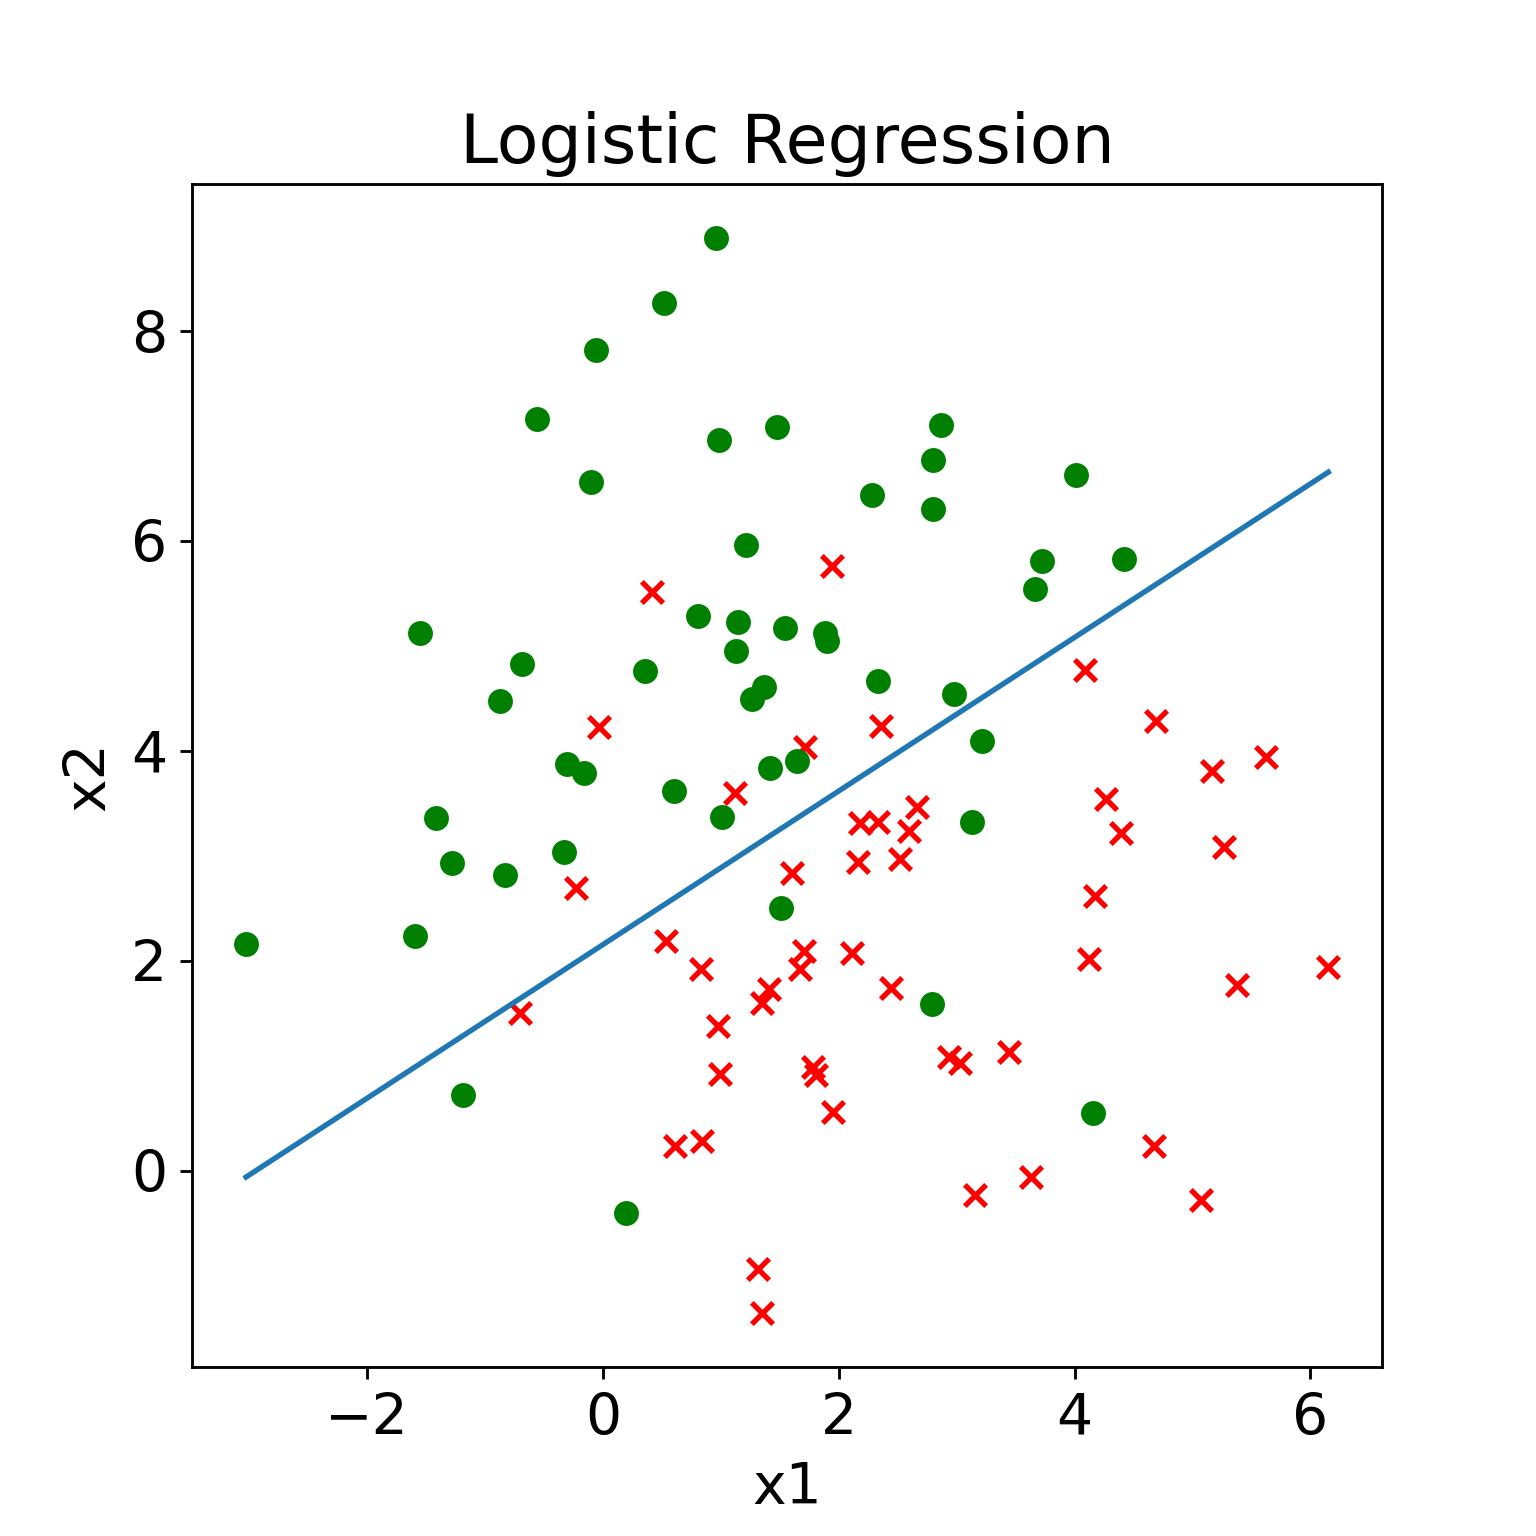
\includegraphics[width=\linewidth]{logistic_regression.png}
\end{figure}
\newpage
\textbf{2 (a)} If we consider only $ w_m $, we can express the log-likelihood as
\[
  \sum_{i=1}^{N} log([p(y^{(i)} = m | x^{(i)}, w)]^{\mathbb{I} \{ y^{(i)} = m \}})
\]
\[
  \sum_{i=1}^{N} \mathbb{I} \{ y^{(i)} = m \} log( [ \frac{
    exp[ w_{m}^{T} \phi(x^{(i)}) ]
  }{
    \sum_{j=1}^{K-1} exp[ w_{j}^{T} \phi(x^{(i)}) ]
  } ] )
\]

$ \nabla w_m l (w) = $
\[
  \sum_{i=1}^{N} \mathbb{I} \{ y^{(i)} = m \} 
  \frac{ \sum_{j=1}^{K-1} exp[ w_{j}^{T} \phi(x^{(i)}) ] }{ exp[ w_{m}^{T} \phi(x^{(i)}) ] }
  [
    \frac{
      exp[ w_{m}^{T} \phi(x^{(i)}) ] \phi(x^{(i)})
    }{
      \sum_{j=1}^{K-1} exp[ w_{j}^{T} \phi(x^{(i)}) ]
    }
    - \frac{
      ( exp[ w_{m}^{T} \phi(x^{(i)}) ] )^2 \phi(x^{(i)})
    }{
      ( \sum_{j=1}^{K-1} exp[ w_{j}^{T} \phi(x^{(i)}) ] )^2
    }
  ]
\]
\[
  = \sum_{i=1}^{N} \mathbb{I} \{ y^{(i)} = m \} 
  [
    \frac{
      \sum_{j=1}^{K-1} exp[ w_{j}^{T} \phi(x^{(i)}) ] exp[ w_{m}^{T} \phi(x^{(i)}) ] \phi(x^{(i)}) 
    }{
      exp[ w_{m}^{T} \phi(x^{(i)}) ] \sum_{j=1}^{K-1} exp[ w_{j}^{T} \phi(x^{(i)}) ]
    }
\]
\[
    - \frac{
      \sum_{j=1}^{K-1} exp[ w_{j}^{T} \phi(x^{(i)}) ]
      ( exp[ w_{m}^{T} \phi(x^{(i)}) ] )^2 \phi(x^{(i)})
    }{
      exp[ w_{m}^{T} \phi(x^{(i)}) ]
      ( \sum_{j=1}^{K-1} exp[ w_{j}^{T} \phi(x^{(i)}) ] )^2
    }
  ]
\]
\[
= \sum_{i=1}^{N} \mathbb{I} \{ y^{(i)} = m \}
[
  \phi(x^{(i)})
    - \frac{
      ( exp[ w_{m}^{T} \phi(x^{(i)}) ] ) \phi(x^{(i)})
    }{
      ( \sum_{j=1}^{K-1} exp[ w_{j}^{T} \phi(x^{(i)}) ] )
    }
]
\]
\[
= \sum_{i=1}^{N} \mathbb{I} \{ y^{(i)} = m \} \phi(x^{(i)})
[
  1 
  - \frac{
      ( exp[ w_{m}^{T} \phi(x^{(i)}) ] )
    }{
      ( \sum_{j=1}^{K-1} exp[ w_{j}^{T} \phi(x^{(i)}) ] )
    }
]
\]
\newpage

\end{document}
